\documentclass{sig-alternate}
\usepackage{color}


\newcommand\todo[1]{\textcolor{red}{(#1)}}
\newcommand\done[1]{\textcolor{green}{(#1)}}

\begin{document}

\title{An Overview of Elastic Cloud Applications}
\subtitle{Technical University of Vienna,\\Advanced Internet Computing Lecture,\\
(Jan 2014)}


\numberofauthors{4}
\author{
\alignauthor
Soodeh Farokhi\titlenote{In alphabetical order}\\ %or put the group leader first, if you wish
       1228800
\alignauthor
Gajo Gajic\\
       0828150
\and
\alignauthor
Martin Kalany\\
       0825673
\alignauthor
Jia Wei\\
       0035204
}
       
\date{\today}

\maketitle
\begin{abstract}
\end{abstract}
%\todo{lots of mistakes and ambiguities}
\done{Improved}
Cloud computing provides access to a virtually unlimited amount of resources. In order to materialize this feature, supporting the elastic deployment of applications it is needed to be supported by the cloud providers. Elasticity, the ability to rapidly scale resources up and down on demand, is one of the main advantages of the cloud paradigm and makes it different to an "advanced outsourcing" solution.
However, there are various challenges in order to predict the elasticity requirements of a given application and several approaches have tackled this issue so far. In this paper, we investigate the state-of-the-art of elastic Cloud applications and describe the requirements for supporting elasticity in the Cloud environment. 

\section{Introduction}
%\todo{lots of mistakes and ambiguities} 
\done{Improved}
Nowadays more and more enterprises have been encouraged to migrate their business applications to a Cloud infrastructures to utilize the core features of Cloud computing. Some of these features are the ability to dynamically increase or decrease computing power on demand, using a more flexible pay-by-usage model in order to reduce costs associated with running and maintaining a private data-center. These costs are significant especially if a high availability and short response times are required. 

Ideally, a Cloud platform is infinitely and instantaneously elastic, meaning that infinite computing resources are available and the scaling up of an application can be done instantaneously. Based on this assumption, an application can be scaled out indefinitely with increasing load without increasing response times \cite{brebner2012your}. However, supporting this scenario is not easy to be solved by Cloud Infrastructure-as-as-Service (IaaS) providers or Platform-as-as-Service (PaaS) providers. Namely, they face serious challenges in order to understand the elasticity characteristics of applications and workloads while having to consider the required capacity of their Cloud platforms.

In this paper, we introduce the current research and commercial solutions for the elasticity issue in Cloud computing. Since the authors had a working experiment with the CloudScale, a middleware to build elastic applications on top of Cloud IaaS, advantages and disadvantages of utilizing it in comparison with other work, will be explained in this paper. The goal of the CloudScale experiment, which was investigated as a course project, was comparing the process of deployment an application, twitter-based sentiment analysis, on top of an IaaS (Amazon EC2\footnote{http://aws.amazon.com/ec2/}) by using CloudScale and without using it directly on a PaaS (Google AppEngine \footnote{https://developers.google.com/appengine/}. It is worth mentioning that, although elasticity is interpreted as the capability of both scaling up and down, while scalability is used more for scaling up, in this paper we use both interchangeable.

The rest of the paper is organized as follows. Section \ref{elasticity-req} discusses the possible ways to provide elastic applications on Cloud as well as the essential features to support it. Then, in Section \ref{sec:rw}, which is the main focus of the paper, the state-of-the-art of elastic Cloud applications is presented in two categories, research work and commercial technologies. In Section \ref{CloudScale}, the features of CloudScale is introduced briefly. Finally, Section \ref{conclusion} concludes the paper.

\section{Elasticity Requirements} \label{elasticity-req}
In general, IaaS or PaaS automatic elasticity in a Cloud environment is typically achieved by using a set of provider-defined rules that govern how and when the service should scale up or down to adapt to a varying application load \cite{vaquero2011dynamically}. These rules are a set of conditions that when met trigger some actions on the infrastructure or platform in order to support dynamic scaling. Existing approaches differ greatly in the abstraction level of this process, e.g. the customization of rules and the degree of automation.

While some approaches allow the user to specify only simple conditions by using fixed predefined set of metrics such as CPU and memory usage, other approaches offers service level metrics (e.g., cost-to-benefit ratio) in order to allow the user to specify more complex conditions that may further be combinations of simple rules. Furthermore, existing approaches differ in the way they behave when the supported conditions are met. Figure \ref{fig:scalabilitymechanisms} depicts possible mechanisms of elasticity support on the level of Cloud IaaS or PaaS \cite{vaquero2011dynamically}.

As represented in Figure \ref{fig:scalabilitymechanisms}, IaaS scaling can roughly be divided in two categories, horizontal and vertical. Horizontal scaling is done by either adding new server replicas and load balancers to distribute the load among more servers, or through %\todo{what does the following mean? Network scaling is no where defined} 
\done{Fixed by referring to Figure 1.} dynamic bandwidth allocation by supporting network scaling. 
Vertical scaling can be achieved by changing the instances on-the-fly\footnote{without rebooting the machine} either by re-sizing (e.g. dedicating more physical resources such as CPU and memory to a running virtual machine (VM)) or replacing this instance %\todo{what? 
\done{Fixed: by adding VM instance}. However, on-the-fly changes of resources dedicated to a VM are not supported by the most common operating systems. Some work like \cite{rodero2010infrastructure} tries to facilitate this process by proposing a new abstraction layer closer to the lifecycle of services, which allows for the automatic application deployment and escalation %\todo{what?}
\done{Fixed: by adding application} depending on the service status (not only on the infrastructure). Their proposed abstraction layer sits on top of various Cloud providers, hence avoiding a potential lock-in and allowing Clouds federation transparently.

Apart from VM scalability, load balancing is also a major elasticity issue that needs to be investigated. A load balancer is required to distribute load as evenly as possible among VMs. For example, Amazon as a commercial public Cloud IaaS provider, already has some strategies for load balancing by replicating VMs via the Elastic Load Balancing feature\footnote{http://aws.amazon.com/autoscaling/}. To sum up, having several servers and the mechanisms to distribute load among them is a necessary step towards scaling a Cloud application \cite{rodero2010infrastructure}. 

However, network scalability \todo{according to  Fig.~\ref{fig:scalabilitymechanisms}, this is only an issue for IaaS} \done{yes, that's why I said for "Cloud data-centers" ;)}is a nearly neglected element that should also be considered \cite{wu2009unified} for Cloud data-centers in order to be able to support application elasticity. It is because as several VMs share the same network, potentially producing a huge increase in the required bandwidth, the network also has to be scalable. 

\done{Fixed: the whole paragraph was ignored and will be discussed in next sections}
%Taking into consideration mechanisms presented in Figure \ref{fig:scalabilitymechanisms}, the CloudScale middleware as well as Aneka\footnote{http://www.manjrasoft.com/products.html} and AppScale\footnote{http://www.appscale.com}, which we will introduce in Section \ref{sec:tools}, fall into the "container replication" category \todo{what is this?} in the platform layer (the container is the CloudScale here) \todo{how is Cloudscale connected to the Aneka and AppScale?}.

\begin{figure*}
\centering
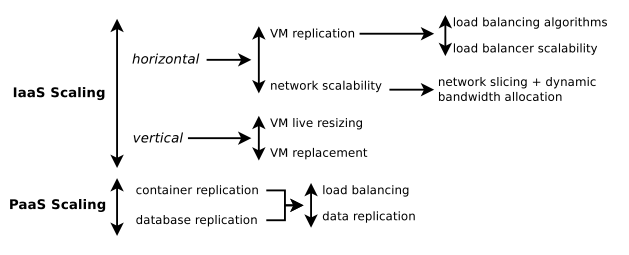
\epsfig{file=figures/ScalabilityMechanisms.png, , width = 11.5cm}
\caption{Possible mechanisms to support elasticity on Cloud IaaS and PaaS \cite{vaquero2011dynamically}.}
\label{fig:scalabilitymechanisms}
\end{figure*}

\section{Related work}
\label{sec:rw}
In the following, we provide an overview of significant work dealing with elastic Cloud applications, in which both scientific research and commercial products, technologies and tools are covered.

\subsection{Scientific research}
\label{sec:scientific}
Keller et.~all \cite{keller2013topology} propose a framework contributes by describing necessary interfaces, features, and data exchanges to deploy complex applications across several Cloud infrastructure services, such as Amazon EC2 in a dynamic and adaptive way \todo{what??} \done{complex applications: I think it is clear}. In the other word \todo{which? PaaS?}\done{word not world :D Typo}, the proposed framework in this work uses high-level interfaces for an adaptation plug-in in order to support elastic applications deployment. These interfaces simplify the retrieval of necessary input data for all placement algorithms and support state-full, or complex application architectures. \todo{what??} \done{Enhanced: is it clear now?}

%Aeolus component model is proposed in \cite{di2012towards} to capture elastic scaling scenario from realistic Cloud deployments, and specifies compositions of services to automate deployments, planning of day-to-day activities such as software upgrade planning, service deployment, and elastic scaling\todo{what??}.

Work presented in \cite{brebner2012your} introduces an elasticity mechanism of a typical Cloud IaaS platform (inspired by Amazon EC2) and presents a Service Oriented Performance Modeling method and tool to model and predict the elasticity characteristics of three realistic applications and workloads on this Cloud platform. The authors compare the pay-as-you-go instance costs and end-user response time for these elasticity scenarios. Their proposed model is able to predict the elasticity requirements (in terms of the maximum instance spin-up time) for the working scenarios \todo{this doesn't really say much} \done{we cannot describe the whole work here, only some clue of their work for a reader}.

The OSGi\footnote{Open Services Gateway initiative}-inspired component framework COSCA \cite {kachele2013component} automatically manages the elastic deployment of component-based applications by isolating components of different applications and hides distribution using a virtualized and distributed OSGi-like framework. It eases the usage of Cloud resources and scalability for component-based applications. 

Han et.~all \cite{han2012lightweight} adopt a lightweight approach along with its algorithm to enable cost-effective elasticity for Cloud applications. The proposed approach operates fine-grained scaling at the resource level (CPUs, memory, I/O) in addition to VM-level scaling to efficiently scale resources up and down in order to meet the given Quality of Service (QoS) requirements while reducing the cost of Cloud providers.

\emph{Orleans} \cite{larus2013look,bykov2011orleans} is a software framework developed at Microsoft Research to build reliable, scalable and elastic Cloud applications. It includes a programming model that encourages the use of simple, easy to understand \todo{what??}\done{read the end: concurrency patterns} and employs concurrency patterns. It is based on distributed actor-like components called grains, which are isolated units of state and computation that communicate through asynchronous messages. \emph{Orleans} enables a developer to concentrate on application logic, while the \emph{Orleans} runtime provides scalability, availability, and reliability.

\subsection{Commercial approaches, technologies and tools}
\label{sec:tools}
Several application provisioning solutions exist, enabling developers and administrators to declaratively specify deployment requirements and dependencies to support repeatable and managed resource provisioning. Some examples are \emph{Opscode Chef}\footnote{www.opscode.com/chef/}, \emph{Puppet}\footnote{http://puppetlabs.com} and \emph{juju}\footnote{http://juju.ubuntu.com}. In juju basic services are described as predefined charms and it can fall into the category in which it supports elastic applications by providing help, hints, or triggers \todo{what?} \done{right, a bit ambiguous. hmmm, maybe more details are needed, if I find any time to do so}.
 
\emph{Aneka} \cite{vecchiola2009aneka} as a .NET-based platform focuses on enabling hybrid Cloud applications, as a composition of two or more Clouds mostly private and public, %\todo{what??} 
\done{Fixed by added Hybrid Clouds definition}
by employing a specialized programming model. It is able to deploy containers and run user applications on several IaaS providers. Aneka similar to Grid computing middleware, provides a relatively low-level abstraction based on the message passing interface (MPI). In general, Aneka seems more suitable for building scientific computing applications than enterprise applications. 

\emph{AppScale} \cite{chohan2009appscale} as an open source extension to the Google AppEngine (GAE) PaaS allows users to build their own GAE compliant PaaS on top of any private or public IaaS service. Namely, it provides a framework to investigate the interaction between PaaS and IaaS systems. To provide elasticity, it scales the VMs used to host containers depending on actual application demand, automatically configuring the load balancers. It targets Online Transaction Processing (OLTP) style enterprise applications.

\emph{Carina Environment Manager}\footnote{https://github.com/blackberry/OpenNebula-Carina} automates and speeds up the deployment of services onto the OpenNebula IaaS platform. It supports the automated creation and run-time scaling of multi-VM application environments according to %\todo{which?} 
\done{Fixed} some policies, which can be defined in a way to control how VMs are added or removed based on manual, time of day, or application load-based triggers. 
%It leverages the OpenNebula contextualization framework to setup clusters of VMs in a master-slave configuration or a set of workers with an IP load-balancer in front.

\emph{CA AppLogic}\footnote{http://www.ca.com/us/Cloud-platform.aspx} is another commercial tool to automate complex application deployment. It scales applications without changing code or architecture. It provides on demand scaling by assigning resources to the service as a single entity, rather than a collection of components.
%CloudBees RUN@Cloud\footnote{http://www.Cloudbees.com/} is a service which provides continuous integration and an elastic platform for hosting Enterprise Java Beans (EJB) applications.

\todo{many, many tools listed, but I don't think we capture the essance} \done{I think for a course paper, it is more than enough to determine the state-of-the-art work which we did it well here!}
%-----------------------------------------------------------------------------------
\section{CloudScale Features} {\label{CloudScale}
In this section, we briefly enumerate the features of CloudScale and compare it with the previous introduced approaches.

CloudScale is used as a middleware to build applications on top of Cloud IaaS by providing an abstraction that makes elastic applications running on top of an IaaS seem like regular, non-distributed Java applications. More precisely, it places a middle layer between IaaS offerings, which provide great control over the application, but with high deployment effort, and PaaS offerings, which are easy to use, but with limited control \cite{leitner2012Cloudscale}. 

In the other word, it allows application developers to have full control over the deployed applications which can not been possible by using a PaaS. Another advantage of CloudScale is in providing an abstract layer so that applications are not bound to any specific Cloud providers. Thus, they are easy to migrate, and work well in private or hybrid Clouds while still providing an abstraction comparable to commercial PaaS solutions. 

Compared to similar approaches for elastic application deployment in Clouds, CloudScale endeavors to be a more general tool to support a wide range of elastic application types, such as data-intense, processing-intense and OLTP style web applications, while other work mostly restrict the types of applications that are supported or usage of proprietary APIs \cite{Leitner2013}.

The main difference between CloudScale and the other similar approaches, as mentioned previously, is providing full control over the applications for the developers. For this purpose, although some scalability-related issues are hidden from developers, they are still free to customize how CloudScale works based on their requirements. This is achieved by implementing custom scaling policies or managing so called Cloud-Objects (regular program-level objects that are abstractions of application logics, and should be distributed over a Cloud) in the application manually \cite{leitner2012Cloudscale}.

\section{Conclusion} 
\label{conclusion}
In this paper we presented an overview of approaches in elastic Cloud applications which include both current scientific research as well as commercial tools. We also elaborated necessary requirements to support elasticity in the Cloud environment. Advantages and disadvantages of CloudScale were discussed, based on the experience gained by the authors related to deploying a twitter-based sentiment analysis application with and without using CloudScale in the Amazon EC2 Cloud (IaaS) and Google AppEngine PaaS.

%bibliography ----------------------------------------------------------------------
\bibliographystyle{abbrv}
\bibliography{sigproc} 
\end{document}
